%%%%%%%%%%%%%%%%%%%%%%%%%%%%%%%%%%%%%%%%%%%%%%%%%%%%%%%%%%%%
% INTRODUCTION
%%%%%%%%%%%%%%%%%%%%%%%%%%%%%%%%%%%%%%%%%%%%%%%%%%%%%%%%%%%%

\section{Introduction}\label{sec:intro}
Partial differential equations (PDEs) are a cornerstone of modern science, underpinning many contemporary physical theories that explain natural phenomena. The ability to solve PDEs grants us the power to predict future states of a system (forward process) and estimate underlying physical properties from state measurements (inverse process).

To date, numerous methods \cite{aliabadi2020boundary,solin2005partial} have been proposed to numerically solve PDEs for both the forward and inverse directions. However, the classical methods can be prohibitively slow, prompting the development of data-driven, learning-based solvers that are significantly faster and capable of handling a family of PDEs. These learning-based approaches \cite{li2020fourier, li2021physics, lu2021learning, raissi2019physics} typically learn a {\em deterministic} mapping between input coefficients and their solutions using deep neural networks. 


Despite the progress, existing learning-based approaches, much like classical solvers, rely on complete observations of the coefficients to map solutions. However, complete information on the underlying physical properties or the state of a system is rarely accessible; in reality, most measurements are sparse in space and time. Both classical solvers and the state-of-the-art data-driven models often overlook these scenarios and consequently fail when confronted with partial observations. This limitation confines their use primarily to synthetic simulations, where full scene configurations are available by design, making their application to real-world cases challenging.

We present a comprehensive framework, DiffusionPDE, for solving PDEs in both forward and inverse directions under conditions of highly partial observations—typically just 1\textasciitilde 3\% of the total information. This task is particularly challenging due to the numerous possible ways to complete missing data and find subsequent solutions. Our approach uses a generative model to formulate the joint distribution of the coefficient and solution spaces, effectively managing the uncertainty and simultaneously reconstructing both spaces. During inference, we sample random noise and iteratively denoise it following standard diffusion models \cite{ho2020denoising}. However, we uniquely guide this denoising process with sparse observations and relevant PDE constraints, generating plausible outputs that adhere to the imposed constraints. Notably, DiffusionPDE can handle observations with arbitrary density and patterns with a single pre-trained generative network.

We conduct extensive experiments to show the versatility of DiffusionPDE as a general PDE-solving framework. We evaluate it on a diverse set of static and temporal PDEs, including Darcy Flow, Poisson, Helmholtz, Burger's, and Navier-Stokes equations. DiffusionPDE significantly outperforms existing state-of-the-art learning-based methods for solving PDEs \cite{li2020fourier, li2021physics, lu2021learning, raissi2019physics,zhao2022learning} in both forward and inverse directions with sparse measurements, while achieving comparable results with full observations. Highlighting the effectiveness of our model, DiffusionPDE accurately reconstructs the complete state of Burgers' equation using time-series data from just five sensors (Fig.~\ref{fig:nonbounded_ns_all}), suggesting the potential of generative models to revolutionize physical modeling in real-world applications.

\begin{figure}[t!]
    \centering
    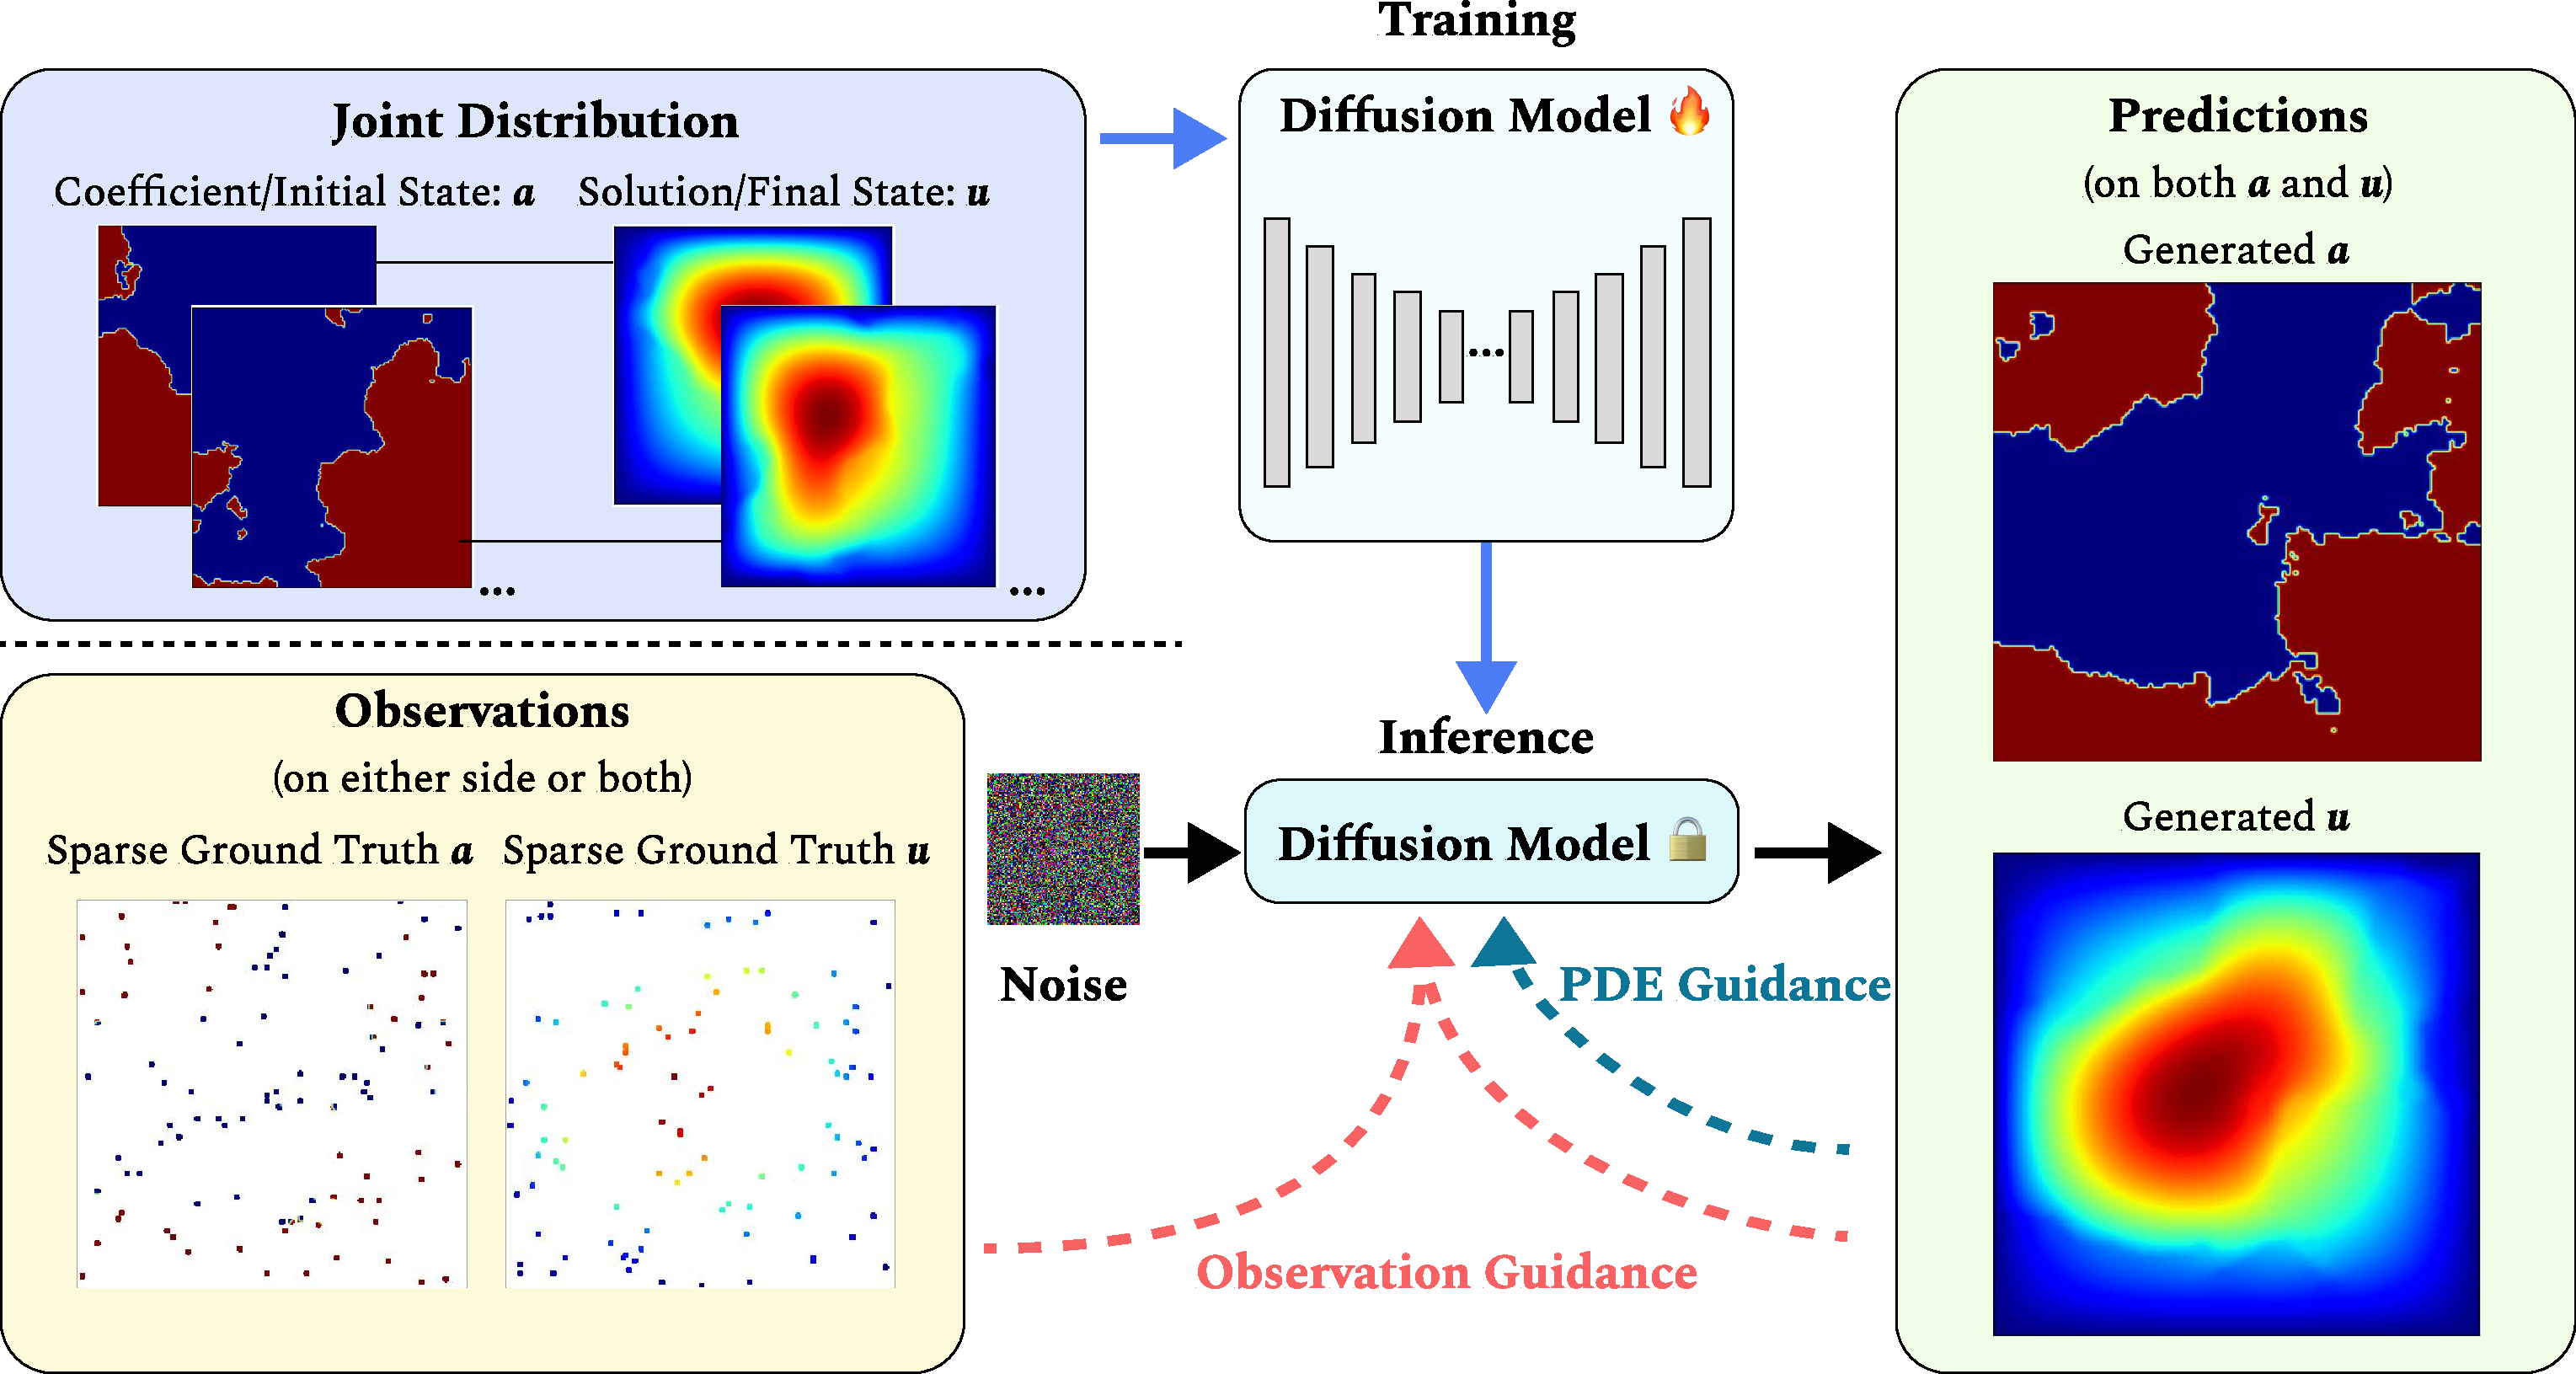
\includegraphics[width=0.99\textwidth]{figs/architecture.pdf}
    \caption{We propose DiffusionPDE, a generative PDE solver under partial observations. Given a family of PDE with coefficient (initial state) $a$ and solution (final state) $u$, we train the diffusion model on the joint distribution of $a$ and $u$. During inference, we gradually denoise a Gaussian noise, guided by sparse observation and known PDE function, to recover the full prediction of both $a$ and $u$ that align well with the sparse observations and the given equation.}
    \label{fig:architecture}
\end{figure}




